\documentclass[a4paper,11pt,fleqn]{article}%fleqn pour aligner les equations à gauche
\usepackage{/home/rweye/Nextcloud/Documents/Overleaf/Styles/Exercice}


\newcommand{\chnum}{Chapitre 4}
\newcommand{\chtitle}{Le noyau de l'atome}
\newcommand{\dtype}{Exercices}

\begin{document}
\maketitle

\begin{multicols}{2}
\section{Vous prendrez bien un verre d'ions ?}
L'eau que nous buvons n'est pas pure. Elle contient de nombreux ions.
\begin{enumerate}
	\item Chercher les numéros atomiques des éléments correspondant aux ions monoatomiques présents dans cette eau.
	\item Calculer le nombre d'ion calcium \ce{^40_20Ca^2+} présents dans \SI{1}{L} de cette eau sachant qu'un ion calcium est un atome de calcium ayant perdu deux électrons.
\end{enumerate}

\textbf{Composition de l'eau d'Evian, minéralisation totale (\unit{\milli\gram\per\liter})}\\
\begin{tabular}{|>{\centering}m{3cm}|>{\centering}m{0.7cm}|>{\centering}m{3.2cm}|>{\centering\arraybackslash}m{0.7cm}|}\hline
\textbf{Calcium \ce{Ca^2+}} &\num{80}&\textbf{Bicarbonate \ce{HCO3-}}&\num{360}\\ \hline
\textbf{Magnésium \ce{Mg^2+}} &\num{26}&\textbf{Sulfate \ce{SO4^2-}}&\num{14}\\ \hline
\textbf{Sodium \ce{Na+}} &\num{6.5}&\textbf{Chlorure \ce{Cl-}}&\num{10}\\ \hline
\textbf{Potassium \ce{K+}} &\num{1}&\textbf{Nitrate \ce{NO3-}}&\num{3.8}\\ \hline
\textbf{Silice \ce{SiO2}} &\num{15}&&\\ \hline
\end{tabular}
\section{Il vient du sol ...}
Le radon, de symbole \ce{Rn} et de numéro atomique $Z=86$, est un gaz radioactif d'origine naturelle. le radon 222 possède 222 nucléons. Il est issu de la désintégration naturelle des noyaux de radium \ce{^226_88Ra} présent, par exemple dans les roches granitiques.
\begin{enumerate}
	\item \begin{enumerate}
		\item Déterminer la composition d'un atome de radon 222.
		\item Déterminer la composition d'un atome de radium 226.
	\end{enumerate}
	\item \begin{enumerate}
		\item Un noyau de radium 226 se désintègre : ses protons et ses neutrons se réorganisent pour former un noyau de radon 222 et un autre noyau. Donner la composition de ce dernier noyau.
		\item Identifier l'écriture conventionnelle de ce noyau parmi celles qui sont données ci-dessous :
		\begin{center}
			\ce{^4_2He} ; \ce{^3_2He} ; \ce{^3_1H} ; \ce{^7_3Li}
		\end{center}
	\end{enumerate}
	\item \begin{enumerate}
		\item Déterminer la masse approchée d'un atome de radon 226.
		\item Dans un bâtiment, le seuil maximal avant l'obligation de travaux d'aération est de 400 désintégrations de radon par \unit{\meter\cubed} et par seconde. Dans une salle de classe de \SI{125}{\meter\cubed}, \SI{4,17E-16}{g} de radon se désintègrent en 10 heures.\\ Déterminer s'il faut envisager des travaux d'aménagement dans cette salle de classe.
	\end{enumerate}
\end{enumerate}
\textbf{Donnée :} $m_{\text{nucléon}}$ = \SI{1,67E-27}{kg}

\section{*Shine*}
Le diamant est un cristal constitué uniquement d'atomes de carbone. On considère que ces atomes sont tous des atomes de carbone 12 ($A$ = 12 nucléons). Il faut en moyenne 20 tonnes de minerai pour extraire \SI{1,0}{g} de diamant, soit \SI{5,0} carats. Le diamant coûte très cher : un diamant de 1,1 carats peut être vendu \SI{15000}{€}.\\
Combien coûte un "atome de diamant" ?

\section{L'atomium de Bruxelles}
L'atomium de Bruxelles a été construit pour l'exposition universelle de 1958.\\

\noindent \colorbox{blue!10}{\begin{minipage}{.6\linewidth}
	L'atomium représente la maille élémentaire d'un cristal de fer agrandie 165 milliards de fois. Il est composé de neuf sphères (une à chaque sommet du cube et une au centre) qui représentent chacune un atome de fer. Chaque sphère a un diamètre d'environ \SI{18}{m} et une masse de \SI{250}{t}.
	\begin{flushright}
		\emph{D'après "Atomium", bruxelles.be}
	\end{flushright}
\end{minipage}}
\begin{minipage}[t]{.4\linewidth}
	\centering
	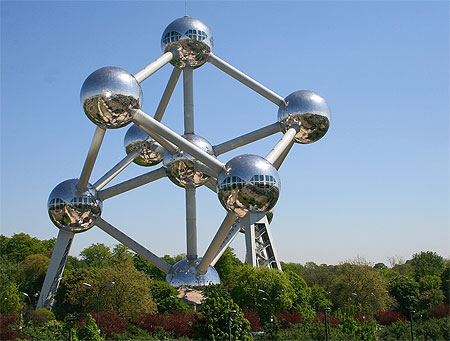
\includegraphics[scale=.2]{Ressources/Atomium.jpg}
\end{minipage}

\begin{enumerate}
	\item Le monument a une hauteur de \SI{102}{m}. La maille de fer représentée dans la même disposition a une hauteur de \SI{560}{pm}. L'échelle annoncée dans le document est-elle respectée ?
\end{enumerate}
L'isotope le plus abondant du fer a pour notation symbolique \ce{^56_26Fe}.
\begin{enumerate}[resume]
	\item Quelle est la masse d'un atome de fer ?
	\item Si les sphères étaient constituées uniquement d'atomes de fer, combien d'atomes chacune\\ contiendrait-elle ?
\end{enumerate}

\section{Le bouclier de Captain America}
Des chercheurs américains de l'université du Nord du Texas (UNT) ont synthétisé un alliage qui serait presque  aussi résistant que le bouclier de Captain America.
\begin{enumerate}
	\item Quel volume de cet alliage est nécessaire pour fabriquer une copie du bouclier de Captain America ?
	\item Quel serait le prix à payer pour une telle copie ?
\end{enumerate}

\noindent \colorbox{orange!10}{\begin{minipage}{\linewidth}
		Bouclier de Captain America dans l'Univers Marvel : 
		\begin{itemize*}
			\item Concepteur : Myron MacLain
			\item Composition alliage de vibranium du Wakanda et d'acier
			\item Dimensions : disque d'environ \SI{76}{cm} de diamètre et \SI{,5}{cm} d'épaisseur
			\item Masse : environ \SI{5}{kg}
		\end{itemize*}
		\begin{flushright}
			\emph{D'après l'articule "Captain America", wikipedia.org}
		\end{flushright}
\end{minipage}}

\noindent \colorbox{red!10}{\begin{minipage}{\linewidth}
\textbf{Données :}
\begin{itemize}
	\item \textbf{Formule de l'alliage :} \ce{Fe42Mn28Co18Cr15Si15}
	\item \textbf{Masse volumique de l'alliage :} $$\rho_{alliage} = \SI{7,13}{\gram\per\centi\meter\cubed} = \SI{7130}{\kilo\gram\per\meter\cubed} $$
	\item \textbf{Éléments composant l'alliage :}
	\end{itemize}

\noindent \begin{tabular}{|>{\centering}m{1.9cm}|>{\centering}m{.9cm}|>{\centering}m{.9cm}|>{\centering}m{.9cm}|>{\centering}m{.9cm}|>{\centering\arraybackslash}m{.9cm}|}
		\hline \textbf{Élément} & \ce{Fe} & \ce{Mn} & \ce{Co} &\ce{Cr} & \ce{Si}\\
		\hline \textbf{Isotope majoritaire} & \ce{^56_26Fe} & \ce{^55_25Mn} & \ce{^52_27Co} &\ce{^52_24Cr} & \ce{^28_14Si}\\
		\hline \textbf{Prix juillet 2016 ($\$/t$)}& \num{57} & \num{1600} &\num{25000} & \num{7100} & \num{1600}\\
		\hline
	\end{tabular}
\end{minipage}}
\end{multicols}
\end{document}